\documentclass[12pt]{extarticle}
\usepackage[letterpaper, left=0.75in, right=0.75in, top=0.8in, bottom=0.8in,
  headheight=20pt, headsep=16pt, footskip=30pt]{geometry}
\usepackage{fontspec}
\setmainfont{texgyreheros}[Extension=.otf, UprightFont=*-regular,
  BoldFont=*-bold, ItalicFont=*-italic, BoldItalicFont=*-bolditalic]
\usepackage{tikz}
\usetikzlibrary{shapes.geometric, arrows.meta}
\usepackage{array}
\usepackage{fancyhdr}
\pagestyle{fancy}
\fancyhf{}
\fancyhead[L]{Week 8 / Rook race and Nim / Grades 4--5}
\fancyfoot[L]{Bellingham Math Circle / Week 8 / F08-U-v4}
\fancyfoot[R]{\thepage}
\renewcommand{\headrulewidth}{0pt}
\setlength{\parindent}{0pt}
\setlength{\parskip}{0pt}
\linespread{1.12}
\hyphenpenalty=10000
\exhyphenpenalty=10000
\newcommand{\prob}[1]{\textbf{Problem #1:}}
\begin{document}
\raggedright
\noindent\begin{minipage}[c]{4.9in}\raggedright
Players take turns. On a board, a move slides the token straight left or straight down, toward the star's side, one or more squares. Whoever moves the token onto the star wins.

\vspace{0.12in}
In a game with piles of counters, a move takes one or more counters from one pile. Whoever takes the last counter wins.
\end{minipage}\hfill\begin{minipage}[c]{1.8in}\raggedleft
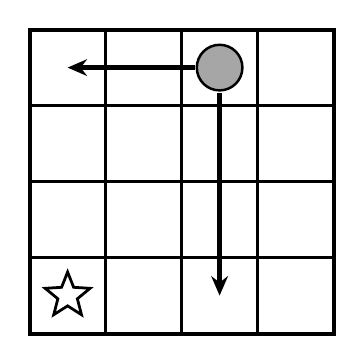
\begin{tikzpicture}[x=1in,y=1in]
\draw[line width=0.9pt] (0,0) grid[step=0.38] (1.5200,1.5200);
\draw[line width=1.4pt] (0,0) rectangle (1.5200,1.5200);
\node[star, star points=5, star point ratio=2.3, draw=black, line width=1.0pt, inner sep=0pt, outer sep=0pt, minimum size=0.236in] at (0.1900,0.1900) {};
\filldraw[fill=black!35, draw=black, line width=0.9pt] (0.9500,1.3300) circle (0.1140);
\draw[-{Stealth[length=7pt,width=6pt]}, line width=1.6pt] (0.8246,1.3300) -- (0.1900,1.3300);
\draw[-{Stealth[length=7pt,width=6pt]}, line width=1.6pt] (0.9500,1.2046) -- (0.9500,0.1900);
\end{tikzpicture}
\end{minipage}

\vspace{0.35in}
\prob{1} Color every square of this 8-by-8 board except the star: green if the first player can always win when the token starts there, red if the second player can always win. Explain why the second player can always win from a red square.

\vspace{0.2in}
\begin{center}
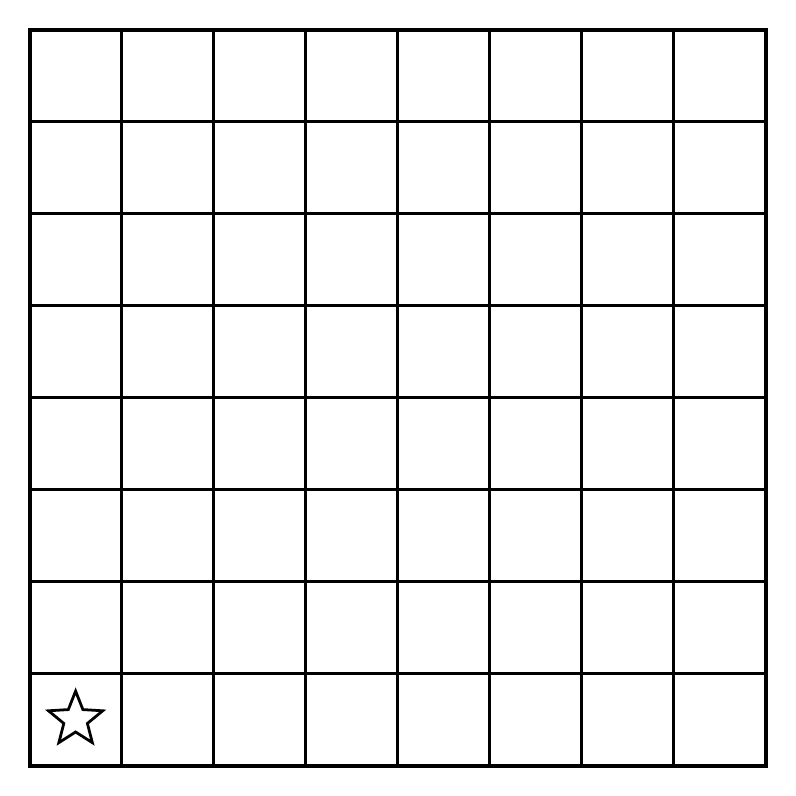
\begin{tikzpicture}[x=1in,y=1in]
\draw[line width=0.9pt] (0,0) grid[step=0.46] (3.6800,3.6800);
\draw[line width=1.4pt] (0,0) rectangle (3.6800,3.6800);
\node[star, star points=5, star point ratio=2.3, draw=black, line width=1.0pt, inner sep=0pt, outer sep=0pt, minimum size=0.285in] at (0.2300,0.2300) {};
\end{tikzpicture}
\end{center}
\newpage
\prob{2} Find two piles of counters that make the same game as this board with the token on the dot. Explain how each move on the board matches a move with the piles. Which player can always win from piles of 23 and 17? From piles of 30 and 30?

\vspace{0.2in}
\begin{center}
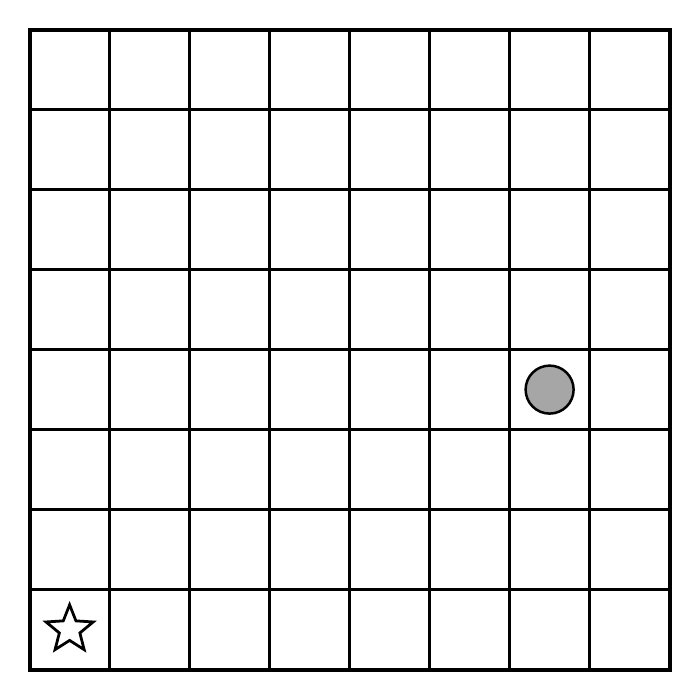
\begin{tikzpicture}[x=1in,y=1in]
\draw[line width=0.9pt] (0,0) grid[step=0.4] (3.2000,3.2000);
\draw[line width=1.4pt] (0,0) rectangle (3.2000,3.2000);
\node[star, star points=5, star point ratio=2.3, draw=black, line width=1.0pt, inner sep=0pt, outer sep=0pt, minimum size=0.248in] at (0.2000,0.2000) {};
\filldraw[fill=black!35, draw=black, line width=0.9pt] (2.6000,1.4000) circle (0.1200);
\end{tikzpicture}
\end{center}
\newpage
\prob{3} Play many games with three piles from each start. Which player can always win?

\vspace{0.25in}
\noindent\hspace{0.3in}\makebox[0.9in][l]{1, 1, 1}\begin{tikzpicture}[x=1in,y=1in]\draw[line width=0.6pt] (0,0) -- (1.6,0);\end{tikzpicture}\hspace{0.6in}\makebox[0.9in][l]{1, 1, 2}\begin{tikzpicture}[x=1in,y=1in]\draw[line width=0.6pt] (0,0) -- (1.6,0);\end{tikzpicture}

\vspace{0.3in}
\noindent\hspace{0.3in}\makebox[0.9in][l]{1, 2, 3}\begin{tikzpicture}[x=1in,y=1in]\draw[line width=0.6pt] (0,0) -- (1.6,0);\end{tikzpicture}\hspace{0.6in}\makebox[0.9in][l]{2, 2, 5}\begin{tikzpicture}[x=1in,y=1in]\draw[line width=0.6pt] (0,0) -- (1.6,0);\end{tikzpicture}

\vspace{0.3in}
\noindent\hspace{0.3in}\makebox[0.9in][l]{1, 3, 4}\begin{tikzpicture}[x=1in,y=1in]\draw[line width=0.6pt] (0,0) -- (1.6,0);\end{tikzpicture}\hspace{0.6in}\makebox[0.9in][l]{1, 4, 5}\begin{tikzpicture}[x=1in,y=1in]\draw[line width=0.6pt] (0,0) -- (1.6,0);\end{tikzpicture}
\vspace{0.6in}

\prob{4} Find all the starts with three piles, each with 1 to 7 counters, where the second player can always win. The order of the piles does not matter.
\newpage
\prob{5} The second player can always win from each of these starts.
\begin{center}1, 2, 3\hspace{0.45in}1, 4, 5\hspace{0.45in}2, 4, 6\hspace{0.45in}3, 5, 6\hspace{0.45in}2, 5, 7\end{center}
The first player can always win from each of these starts.
\begin{center}1, 2, 4\hspace{0.45in}2, 3, 5\hspace{0.45in}2, 4, 7\hspace{0.45in}3, 4, 6\end{center}
Make these starts with counters, and split every pile into stacks of 1, 2, 4, 8, 16 and so on, with no two stacks in one pile the same size. Find a rule about the stacks that tells which player can always win.

\vspace{4.0in}

\prob{6} Which player can always win from each of these starts? When it is the first player, find a first move that lets the first player always win.

\vspace{0.3in}
\noindent\hspace{0.3in}\makebox[1.2in][l]{3, 5, 7}\begin{tikzpicture}[x=1in,y=1in]\draw[line width=0.6pt] (0,0) -- (4.6,0);\end{tikzpicture}

\vspace{0.32in}
\noindent\hspace{0.3in}\makebox[1.2in][l]{6, 10, 12}\begin{tikzpicture}[x=1in,y=1in]\draw[line width=0.6pt] (0,0) -- (4.6,0);\end{tikzpicture}

\vspace{0.32in}
\noindent\hspace{0.3in}\makebox[1.2in][l]{13, 9, 7}\begin{tikzpicture}[x=1in,y=1in]\draw[line width=0.6pt] (0,0) -- (4.6,0);\end{tikzpicture}

\vspace{0.32in}
\noindent\hspace{0.3in}\makebox[1.2in][l]{11, 14, 21}\begin{tikzpicture}[x=1in,y=1in]\draw[line width=0.6pt] (0,0) -- (4.6,0);\end{tikzpicture}
\newpage
\prob{7} Explain why your rule from Problem 5 is right for every start, even with piles of hundreds of counters.
\newpage
\noindent\begin{minipage}[t]{4.7in}\vspace{0pt}\raggedright
\prob{8} In a new game, the token may also slide diagonally down and to the left, one or more squares. Color every square of this 8-by-8 board except the star: green if the first player can always win when the token starts there, red if the second player can always win.
\end{minipage}\hfill\begin{minipage}[t]{1.9in}\vspace{0pt}\raggedleft
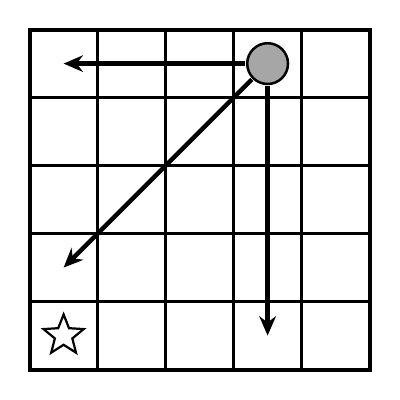
\begin{tikzpicture}[x=1in,y=1in]
\draw[line width=0.9pt] (0,0) grid[step=0.34] (1.7000,1.7000);
\draw[line width=1.4pt] (0,0) rectangle (1.7000,1.7000);
\node[star, star points=5, star point ratio=2.3, draw=black, line width=0.8pt, inner sep=0pt, outer sep=0pt, minimum size=0.211in] at (0.1700,0.1700) {};
\filldraw[fill=black!35, draw=black, line width=0.9pt] (1.1900,1.5300) circle (0.1020);
\draw[-{Stealth[length=7pt,width=6pt]}, line width=1.6pt] (1.0778,1.5300) -- (0.1700,1.5300);
\draw[-{Stealth[length=7pt,width=6pt]}, line width=1.6pt] (1.1900,1.4178) -- (1.1900,0.1700);
\draw[-{Stealth[length=7pt,width=6pt]}, line width=1.6pt] (1.1107,1.4507) -- (0.1700,0.5100);
\end{tikzpicture}
\end{minipage}

\vspace{0.3in}
\begin{center}
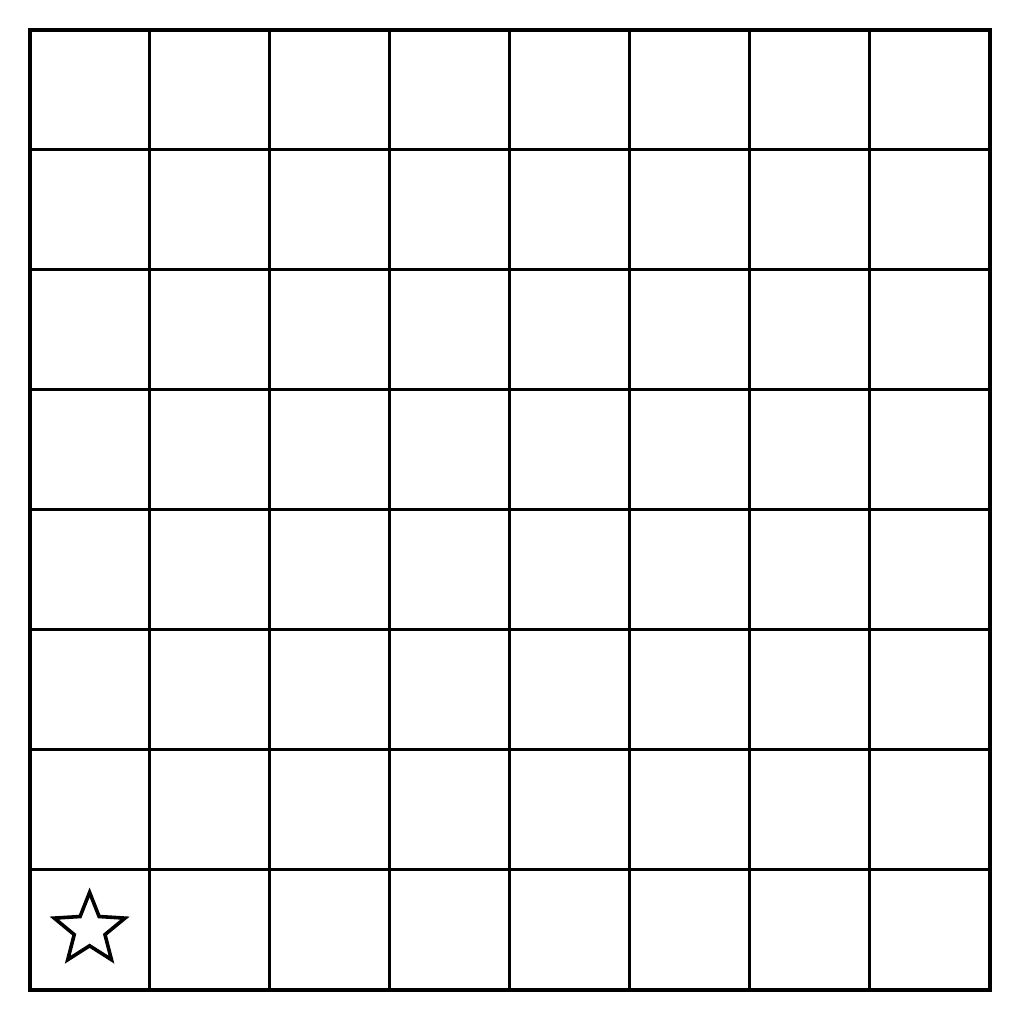
\begin{tikzpicture}[x=1in,y=1in]
\draw[line width=0.9pt] (0,0) grid[step=0.6] (4.8000,4.8000);
\draw[line width=1.4pt] (0,0) rectangle (4.8000,4.8000);
\node[star, star points=5, star point ratio=2.3, draw=black, line width=1.3pt, inner sep=0pt, outer sep=0pt, minimum size=0.372in] at (0.3000,0.3000) {};
\end{tikzpicture}
\end{center}
\newpage
\prob{9} In the game from Problem 8, mark all the red squares on this 20-by-20 board. Explain how you know you have found them all.

\vspace{0.2in}
\begin{center}

\begin{tikzpicture}[x=1in,y=1in]
\draw[line width=0.5pt] (0,0) grid[step=0.3] (6.0000,6.0000);
\draw[line width=1.4pt] (0,0) rectangle (6.0000,6.0000);
\node[star, star points=5, star point ratio=2.3, draw=black, line width=0.8pt, inner sep=0pt, outer sep=0pt, minimum size=0.186in] at (0.1500,0.1500) {};
\end{tikzpicture}
\end{center}

\end{document}
